\documentclass{article}\usepackage[]{graphicx}\usepackage[]{color}
% maxwidth is the original width if it is less than linewidth
% otherwise use linewidth (to make sure the graphics do not exceed the margin)
\makeatletter
\def\maxwidth{ %
  \ifdim\Gin@nat@width>\linewidth
    \linewidth
  \else
    \Gin@nat@width
  \fi
}
\makeatother

\definecolor{fgcolor}{rgb}{0.345, 0.345, 0.345}
\newcommand{\hlnum}[1]{\textcolor[rgb]{0.686,0.059,0.569}{#1}}%
\newcommand{\hlstr}[1]{\textcolor[rgb]{0.192,0.494,0.8}{#1}}%
\newcommand{\hlcom}[1]{\textcolor[rgb]{0.678,0.584,0.686}{\textit{#1}}}%
\newcommand{\hlopt}[1]{\textcolor[rgb]{0,0,0}{#1}}%
\newcommand{\hlstd}[1]{\textcolor[rgb]{0.345,0.345,0.345}{#1}}%
\newcommand{\hlkwa}[1]{\textcolor[rgb]{0.161,0.373,0.58}{\textbf{#1}}}%
\newcommand{\hlkwb}[1]{\textcolor[rgb]{0.69,0.353,0.396}{#1}}%
\newcommand{\hlkwc}[1]{\textcolor[rgb]{0.333,0.667,0.333}{#1}}%
\newcommand{\hlkwd}[1]{\textcolor[rgb]{0.737,0.353,0.396}{\textbf{#1}}}%
\let\hlipl\hlkwb

\usepackage{framed}
\makeatletter
\newenvironment{kframe}{%
 \def\at@end@of@kframe{}%
 \ifinner\ifhmode%
  \def\at@end@of@kframe{\end{minipage}}%
  \begin{minipage}{\columnwidth}%
 \fi\fi%
 \def\FrameCommand##1{\hskip\@totalleftmargin \hskip-\fboxsep
 \colorbox{shadecolor}{##1}\hskip-\fboxsep
     % There is no \\@totalrightmargin, so:
     \hskip-\linewidth \hskip-\@totalleftmargin \hskip\columnwidth}%
 \MakeFramed {\advance\hsize-\width
   \@totalleftmargin\z@ \linewidth\hsize
   \@setminipage}}%
 {\par\unskip\endMakeFramed%
 \at@end@of@kframe}
\makeatother

\definecolor{shadecolor}{rgb}{.97, .97, .97}
\definecolor{messagecolor}{rgb}{0, 0, 0}
\definecolor{warningcolor}{rgb}{1, 0, 1}
\definecolor{errorcolor}{rgb}{1, 0, 0}
\newenvironment{knitrout}{}{} % an empty environment to be redefined in TeX

\usepackage{alltt}
\usepackage[hmargin = 1in]{geometry}
\usepackage{enumitem}
\usepackage{amsmath, amsthm, amssymb, amsfonts}
\setlist[2]{
font = \color{black},
before = {\color{red}}
}
\usepackage{textcomp}
\IfFileExists{upquote.sty}{\usepackage{upquote}}{}
\begin{document}





\begin{center} \LARGE
Homework 11
\end{center}
\begin{center} \Large
Due April 16, 2020 at 11:59 PM 
\end{center}



\begin{enumerate}
	\item P. 674: 1 (ignore (e), (g)) (10 points for (b), 8 points for others), dataset: {\tt polyol.jmp} 
	
	\begin{itemize}
	\item[(a)]
	

  
  
  $s_{LF} = 67.01$. Thus measures the baseline variation in the molecular weight that would be observed for any fixed pot temperature, assuming the SLR model is appropriate.
  
  \item[(b)] The residuals versus $x$ and the standard residual versus $x$ plots are almost the same. 
  
\begin{knitrout}
\definecolor{shadecolor}{rgb}{0.969, 0.969, 0.969}\color{fgcolor}

{\centering 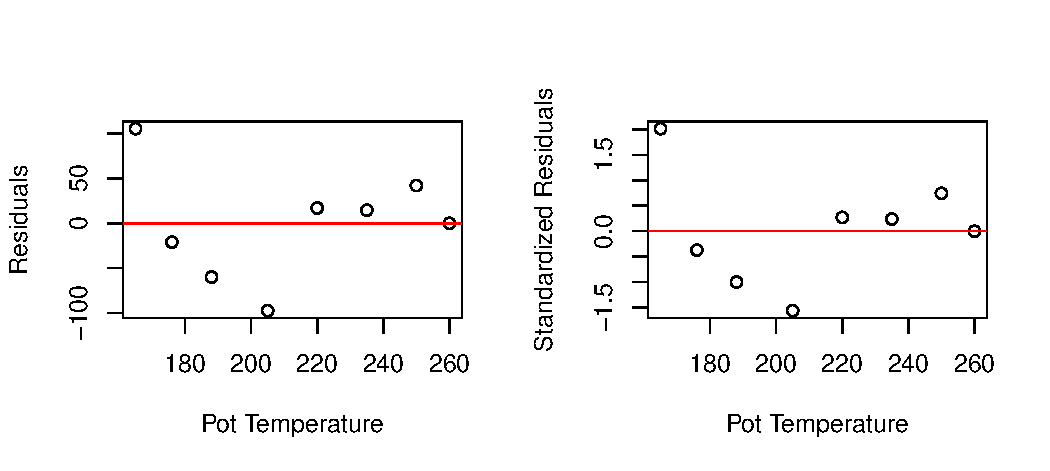
\includegraphics[width=0.8\textwidth]{figure/unnamed-chunk-3-1} 

}



\end{knitrout}
  
  \item[(c)]
  For a 90\% two-sided confidence interval, we use $t_{n-2, 1 - \alpha/2} = t_{6, 0.95} = 1.943$. We calculate $\bar{x} = 212.375, \sum_{i}(x_i - \bar{x})^2 = 8469.875$. So we have
  \begin{align*}
  &b_1 \pm t_{n-2, 1 - \alpha/2} \frac{s_{LF}}{\sqrt{\sum_{i} (x_i - \bar{x})}}\\
  = & 23.49827 \pm 1.943 \frac{67.01}{\sqrt{8469.875}}\\
   =& (22.08, 24.91)
  \end{align*}
  
  \item[(d)]
  For a 90\% two-sided confidence interval, we use $t_{n-2, 1 - \alpha/2} = t_{6, 0.95} = 1.943$. 
  
  So for the mean at $x = 212$, 
  \begin{align*}
  & b_0 + b_1 x \pm t_{n-2, 1 - \alpha/2} s_{LF} \sqrt{\frac{1}{n} + \frac{(x - \bar{x})^2}{\sum_{i} (x_i - \bar{x})^2}}\\
  = & 1807.063 \pm 1.942 \cdot 67.01 \sqrt{\frac{1}{8} + \frac{0.140625}{8469.875}}\\
  =& (1761.03, 1853.10)
  \end{align*}
  
  For the mean at $x = 250$, 
  \begin{align*}
  & b_0 + b_1 x \pm t_{n-2, 1 - \alpha/2} s_{LF} \sqrt{\frac{1}{n} + \frac{(x - \bar{x})^2}{\sum_{i} (x_i - \bar{x})^2}}\\
  = & 2699.997 \pm 1.942 \cdot 67.01 \sqrt{\frac{1}{8} + \frac{1415.641}{8469.875}}\\
  =& (2629.63, 2770.37)
  \end{align*}
  
  \item[(f)]
  For a 90\% one-sided prediction interval, we use $t_{n-2, 1 - \alpha} = t_{6, 0.9} = 1.440$. 
  
  So at $x = 212$, the lower prediction bound is
  \begin{align*}
  & b_0 + b_1 x - t_{n-2, 1 - \alpha} s_{LF} \sqrt{1 + \frac{1}{n} + \frac{(x - \bar{x})^2}{\sum_{i} (x_i - \bar{x})^2}}\\
  = & 1807.063  - 1.440 \cdot 67.01 \sqrt{1 + \frac{1}{8} + \frac{0.140625}{8469.875}}\\
  = & 1704.72
  \end{align*}
  
  For $x = 250$,
  \begin{align*}
  & b_0 + b_1 x - t_{n-2, 1 - \alpha} s_{LF} \sqrt{1 + \frac{1}{n} + \frac{(x - \bar{x})^2}{\sum_{i} (x_i - \bar{x})^2}}\\
  = & 2699.997 - 1.440 \cdot 67.01 \sqrt{1 + \frac{1}{8} + \frac{1415.641}{8469.875}}\\
  =& 2590.31
  \end{align*}
  
  \item[(h)]
  The ANOVA table is
  \begin{center}
  \begin{tabular}{lllll}
  \hline 
  Source & SS & df & MS & F\\ \hline
  Regression & 4676798 & 1 & 4676798 & 1041.58\\
  Error & 26941 & 6 & 4490 & \\ \hline
  Total & 4703739 & 7 & & \\ \hline
  
  \end{tabular}
  \end{center}
  The p-value is
  \[P(F_{1, 6} > 1041.58)\]
  which is less than 0.001, according to Table B.6E, the 0.999 quantile of $F_{1,6}$ is $35.51 < 1041.58$. This is overwhelming evidence that the mean average molecular weight is related to the pot temperature.
  
	\end{itemize}
	
\end{enumerate}
%\newpage 
%\nocite{*}
%\bibliographystyle{plainnat} 
%\bibliography{}
\end{document}
